\chapter{Results}

By expanding the microarchitecture from Exercise 1 \cite{compendium} with a forwarder, pipeline registers, hazard detection and improved ALU, PC and control modules, we succeeded in implementing a pipelined, multi-cycle, MIPS-like processor.
Each component was tested with individual testbenches.
The system as a whole was tested using an end-to-end testbench, as well as by uploading the bitfile to an FPGA in the lab and verifying correctness using the \texttt{hostcomm} utility.
We succeeded in implementing support for the instructions listed as requirements in the exercise description.

\section{Testing in ISim}
Testsbenches for the all modules except the pipeline registers were written and run is ISim. 

\section{Testing on the FPGA}
When the system had been tested thoroughly in ISim, a bitfile was generated, and uploaded to an FPGA, via Hostcomm. The FPGA's instruction memory is loaded with the code in Listing \ref{lst:testcode}. Figure \ref{fig:hostcomm} shows the result of a successful execution on our design. The correctness of the test is ensured by comparing the data memory loaded from the FPGA, after it has run for a short time, with the comments in Listing \ref{lst:testcode} that states "Saving value ...".

\begin{figure}[h!]
    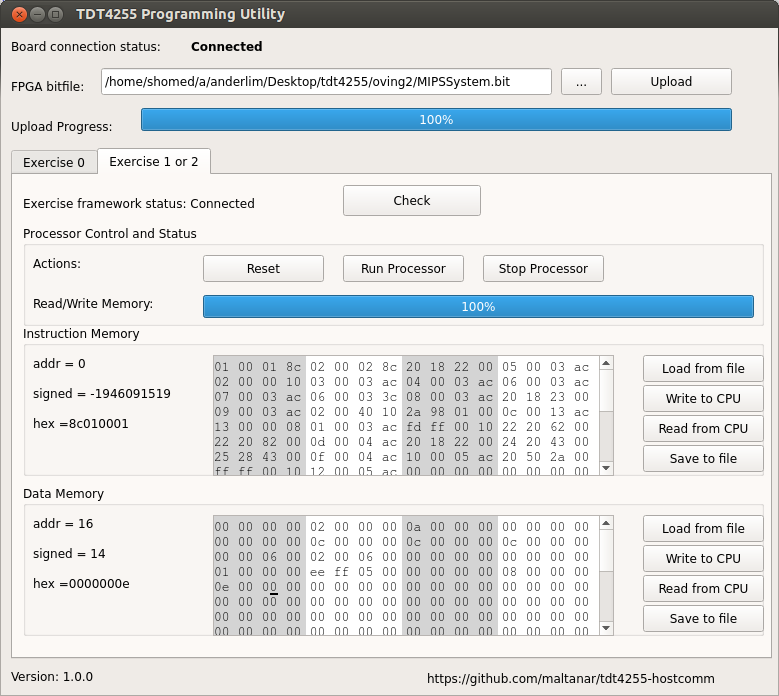
\includegraphics[width=\linewidth]{img/hostcomm_result.png}
    \caption{A screenshot of the hostcomm utility after allowing our processor to execute a the test program.}
    \label{fig:hostcomm}
\end{figure}